\documentclass[preprint,12pt,authoryear]{elsarticle}

\usepackage[utf8]{inputenc}
\usepackage[T1]{fontenc}
\usepackage{lmodern}
\usepackage{amsmath,amssymb,amsthm}
\usepackage{booktabs}
\usepackage{graphicx}
\usepackage[colorlinks=true,linkcolor=blue!50!black,citecolor=blue!50!black,urlcolor=blue!50!black]{hyperref}

\graphicspath{{fig/}}
\newtheorem{proposition}{Proposition}
\newcommand{\todo}[1]{\textcolor{red}{[#1]}}

\journal{Structural Change and Economic Dynamics}

\begin{document}

\begin{frontmatter}

\title{Is learning efficiency a parameter? An agent-based approach to intergenerational knowledge transmission and the AI skill cliff}

\author[lille]{Federico Bassi}
\author[aff2]{\todo{Nome Cognome}\corref{cor}}
\cortext[cor]{Corresponding author.}
\affiliation[lille]{organization={Centre lillois d'\'etudes et de recherches sociologiques et \'economiques (Cler\-s\'e), Universit\'e de Lille \todo{da verificare}},country={France}}
\affiliation[aff2]{organization={\todo{Affiliazione}},country={Italy}}

\begin{abstract}
Growth models in the tradition of \citet{Lucas1988} treat the efficiency with which workers accumulate human capital as a fixed parameter, while the literature on knowledge diffusion \citep{LucasMoll2014,Jarosch2021} locates learning in encounters between workers who know more and workers who know less. Recent evidence that generative AI reduces the employment of entry-level workers \citep{Brynjolfsson2025,HosseiniLichtinger2025} turns this distinction into a policy question: if AI substitutes for junior work, it may also remove the occasions on which junior workers learn from senior ones. This paper develops an agent-based model in which learning efficiency is not assumed but emerges from junior--senior meetings, and uses it to characterise the timing of the resulting losses. Calibrated to an age--wage profile that rises slowly and flattens, as in the Italian private sector, the model shows that a permanent reduction in meetings leaves the human capital of senior workers \emph{exactly} unchanged for a number of years equal to the distance between the junior and senior thresholds, and erodes it thereafter through a cumulative, intergenerational mechanism. We call this delayed fall in aggregate human capital the \emph{skill cliff}. A mean-field identity links the micro-level rules to an aggregate law of motion in which learning efficiency depends on meeting opportunities, on mentoring capacity and on the distribution of knowledge.
\end{abstract}

\begin{keyword}
Human capital \sep Knowledge diffusion \sep Artificial intelligence \sep Agent-based model \sep Mentoring \sep Skill cliff
\JEL C63 \sep J24 \sep O33 \sep O41 \sep J11
\end{keyword}

\end{frontmatter}

% ---------------------------------------------------------------------------
\section{Introduction}

Assumptions about the efficiency of learning are central to theories of growth driven by human capital. The debate can be summarised by two positions. In the canonical formulation of \citet{Lucas1988}, human capital grows as $\dot h = B\,u\,h$, where $u$ is the share of time devoted to learning and $B$ is a technological parameter; in the diffusion approach of \citet{LucasMoll2014}, knowledge is acquired through meetings, and what a learner gains depends on the distance between what the learner knows and what the counterpart knows. Empirical work on coworker learning supports the second view: wage growth is faster for workers whose colleagues earn more, and the value of this learning amounts to a non-negligible share of compensation \citep{Jarosch2021,Herkenhoff2024}.

The distinction is not merely formal. If $B$ is a parameter, a technology that changes the organisation of work leaves the efficiency of learning untouched. If instead $B$ emerges from meetings, a technology that reduces the number of meetings reduces $B$ itself. Generative AI provides a pressing case. Early evidence suggests that it reduces the employment of young and entry-level workers in exposed occupations, while leaving senior employment broadly unchanged \citep{Brynjolfsson2025,HosseiniLichtinger2025}; and recent theoretical work argues that automation may weaken the apprenticeship channel through which tacit knowledge is transmitted across generations \citep{Ide2025}. Whether AI acts as a substitute or as a complement to labour \citep{Acemoglu2024,AcemogluRestrepo2019} then matters not only for current employment, but for the human capital of future senior workers.

The existing literature, however, is lacking in three respects. First, learning efficiency is typically treated as a parameter, even where its microfoundations are explicitly social. Second, the effects of AI on the labour market are measured at impact---on the employment of young workers today---while the transmission channel operates with a delay of one professional generation. Third, the timing of this delay, and the conditions under which a gradual reduction in meetings turns into an abrupt fall in aggregate human capital, have not, to our knowledge, been characterised.

We therefore develop an agent-based model (ABM) in which $B$ is an emergent property of junior--senior meetings, in the spirit of the use of agent-based methods to microfound aggregate dynamics in \citet{Bassi2022} and \citet{RailsbackGrimm2011}. The contribution of the paper is threefold. First, we show that a parsimonious model with demography, meetings and life-cycle learning reproduces a concave age--wage profile and produces a value of the learning share of junior wage growth consistent with \citet{Jarosch2021}. Second, we show that a permanent reduction in meeting opportunities produces a \emph{skill cliff}: senior human capital is exactly unaffected for $s_S - s_J + 1$ years, where $s_J$ and $s_S$ are the junior and senior experience thresholds, and declines thereafter as cohorts trained under fewer meetings become the teachers of the next ones. Third, we derive a mean-field identity that maps the micro-level rules into an aggregate law of motion for $B$, which can be used to augment single-equation growth models.

The remainder of the paper is organised as follows. Section~\ref{sec:background} reviews the theoretical background. Section~\ref{sec:model} presents the model as implemented. Section~\ref{sec:results} reports the baseline simulations and a mechanism experiment that isolates the meeting channel. Section~\ref{sec:aggregate} derives the implications for aggregate modelling. Section~\ref{sec:conclusions} concludes and outlines the introduction of AI.

% ---------------------------------------------------------------------------
\section{Theoretical background and motivation}\label{sec:background}

\paragraph{Learning efficiency as a parameter} In \citet{Lucas1988} the parameter $B$ governs the return to time spent learning and, through it, the growth rate of the economy. Life-cycle models of investment in human capital \citep{BenPorath1967} explain why individual learning declines with age, and hence why empirical age--earnings profiles are concave \citep{MurphyWelch1990,Lagakos2018}; but they too treat the productivity of learning as given.

\paragraph{Learning through meetings} \citet{LucasMoll2014} replace the parameter with a process: agents meet others and adopt their knowledge if it is better. The gain from a meeting is increasing in the knowledge gap, so that the efficiency of learning depends on the distribution of knowledge in the population. \citet{Jarosch2021} estimate that learning from coworkers accounts for 4 to 9 per cent of total compensation, and that it is concentrated in interactions with more knowledgeable colleagues.\footnote{The mapping between their measure and ours is approximate: they measure learning from all coworkers as a share of the compensation of all workers, while we measure learning of junior workers from senior ones as a share of junior wages.}

\paragraph{Automation, entry-level work and the apprenticeship channel} If senior workers transmit tacit knowledge mainly through joint work with junior ones, a technology that automates junior tasks reduces the occasions for transmission \citep{Ide2025}. The available evidence measures the first-round effect: employment of 22--25 year-olds in AI-exposed occupations has fallen by 13--16 per cent relative to older workers \citep{Brynjolfsson2025}, and firms adopting generative AI hire fewer junior workers \citep{HosseiniLichtinger2025}. The second-round effect---on the human capital of those who will be senior workers in ten or twenty years---is, by construction, not yet observable. A model is needed to discipline expectations about it.

% ---------------------------------------------------------------------------
\section{The model}\label{sec:model}

\subsection{Agents and demography}

The economy is populated by $N=5{,}000$ workers indexed by $i$. Each period corresponds to one year. Worker $i$ is characterised by age $a_i$, years of experience $s_i$, a skill level $q_i\in\{L,H\}$ and human capital $h_i$. At the beginning of each period all workers age by one year; those reaching the retirement age $\bar a=65$ leave and are replaced one-for-one by entrants, so that $N$ is constant.\footnote{A variant with the Italian age pyramid, in which $N$ varies over time, is left to a dedicated case study.} An entrant is high-skilled with probability $q=0.3$, enters at age 25 if high-skilled and 20 otherwise, and draws
\begin{equation}
h_{i,0} = \bar h_0(q_i)\, e^{\varepsilon_i}, \qquad \varepsilon_i \sim \mathcal N\!\left(-\tfrac{\sigma^2}{2},\sigma^2\right),
\end{equation}
with $\bar h_0(L)=1$, $\bar h_0(H)=1.5$ and $\sigma=0.2$. Roles are defined by experience rather than age: worker $i$ is \emph{junior} if $s_i < s_J$ and \emph{senior} if $s_i \ge s_S$, with $s_J=5$ and $s_S=15$.

\subsection{Meetings}

Let $J_t$ and $S_t$ denote the number of junior and senior workers. Each senior can follow at most $\kappa$ juniors per year, so that the number of meetings is $\min(pJ_t,\kappa S_t)$ and the probability that a junior meets a senior is
\begin{equation}\label{eq:peff}
p^{\mathrm{eff}}_t = \min\!\left(p,\ \kappa \frac{S_t}{J_t}\right).
\end{equation}
A junior $j$ who meets a senior $k$, drawn uniformly among seniors, gains
\begin{equation}\label{eq:meeting}
\Delta h^{\mathrm{inc}}_{j,t} = \beta \max\left(0,\ h_{k,t}-h_{j,t}\right),
\end{equation}
as in \citet{LucasMoll2014}: the gain is proportional to the knowledge gap, and nothing is unlearned from a less knowledgeable senior. The senior bears no cost.

\subsection{Autonomous learning and obsolescence}

All workers also learn autonomously, at a rate that declines with experience as in \citet{BenPorath1967}, and lose a fraction $d$ of their knowledge to obsolescence:
\begin{equation}\label{eq:aut}
\Delta h^{\mathrm{aut}}_{i,t} = \left[\delta(s_i)-d\right] h_{i,t}, \qquad \delta(s) = \delta_0 \max\!\left(0,\ 1-\frac{s}{S_h}\right).
\end{equation}
Both components are computed on beginning-of-period human capital and applied simultaneously; $h$ remains non-negative because $d<1$.

\subsection{Output, wages and emergent learning efficiency}

Output is $Y_t=\sum_i h_{i,t}$ and wages equal marginal products, $w_i = h_i$.\footnote{Output becomes $Y_t = f(\sum_i h_{i,t}, A_t)$ in the extension with AI.} Emergent learning efficiency is measured as the mean growth rate of junior human capital,
\begin{equation}\label{eq:B}
B_t = \underbrace{\frac{1}{J_t}\sum_{j}\frac{\Delta h^{\mathrm{inc}}_{j,t}}{h_{j,t}}}_{B^{\mathrm{inc}}_t} + \underbrace{\frac{1}{J_t}\sum_{j}\frac{\Delta h^{\mathrm{aut}}_{j,t}}{h_{j,t}}}_{B^{\mathrm{aut}}_t},
\end{equation}
which coincides with $\dot h/h = B\,u$ in \citet{Lucas1988} with $u=1$.

\subsection{Calibration and implementation}

Table~\ref{tab:params} reports the parameter values. Demographic parameters reflect the Italian labour market; $\beta$ is chosen so that $B^{\mathrm{inc}}$ falls within the range estimated by \citet{Jarosch2021}; $(\delta_0,S_h,d)$ are chosen to produce an age--wage profile that rises slowly, peaks late and declines only mildly. The model is implemented in vectorised Python; each run includes a burn-in of 120 years, and statistics are averaged over 30 replications with independent seeds and 95\% confidence intervals. Scenarios share random numbers replication by replication. An independent re-implementation of the same rules with one object per agent in Mesa yields statistically indistinguishable results (Appendix~\ref{app:docking}), a form of model docking \citep{Axtell1996}. Code and data are available at \url{https://github.com/ViciusLio/skill-cliff-abm}.

\begin{table}[t]\centering\small
\caption{Parameters of the baseline model.}\label{tab:params}
\begin{tabular}{@{}l l p{0.29\linewidth} p{0.24\linewidth}@{}}
\toprule
Parameter & Value & Description & Source / criterion \\
\midrule
$N$ & 5{,}000 & workers & --- \\
entry age & 20 / 25 & low / high skill & Italian graduates enter late \\
$\bar a$ & 65 & retirement age & effective exit age, Italy 2024 \\
$q$ & 0.30 & share of high-skilled entrants & tertiary share, age 25--34 \\
$\bar h_0(L),\bar h_0(H)$ & 1.0 / 1.5 & mean entry human capital & normalisation \\
$\sigma$ & 0.20 & dispersion of entry $h$ & arbitrary \\
$s_J$ / $s_S$ & 5 / 15 & junior / senior thresholds & entry-level evidence \\
$p$ & 0.60 & meeting probability & arbitrary (with $\beta$) \\
$\kappa$ & 0.20 & mentoring capacity & arbitrary \\
$\beta$ & 0.10 & meeting effectiveness & $B^{\mathrm{inc}}\in[4\%,9\%]$ \\
$\delta_0, S_h, d$ & 0.04 / 50 / 0.012 & autonomous learning, obsolescence & concave profile \\
\bottomrule
\end{tabular}
\end{table}

% ---------------------------------------------------------------------------
\section{Simulation results}\label{sec:results}

\subsection{Baseline: stylised facts}

The baseline reproduces a concave age--wage profile (Figure~\ref{fig:profile}). Wages peak after 34 years of experience for both skill groups, at a level 1.90 (low-skilled) and 1.72 (high-skilled) times the entry wage, and decline by 3.7 and 0.9 per cent respectively before retirement. Emergent learning efficiency is $B=0.0709$ (95\% CI $[0.0708, 0.0710]$), of which $B^{\mathrm{inc}}=0.0445$, or 63 per cent, comes from meetings (Figure~\ref{fig:B}, panel a). The ratio of seniors to juniors is 5.70, so that mentoring capacity does not bind in the steady state ($p^{\mathrm{eff}}=p$).

Two discrepancies should be noted. First, the profile of low-skilled workers is steeper than that of high-skilled workers, while the evidence points in the opposite direction \citep{Lagakos2018}: juniors are matched to seniors drawn from the whole population, so that low-skilled juniors face a larger gap to close. Second, the wage Gini coefficient (0.135) is well below observed values, because human capital is the only determinant of wages in the model. Neither is a calibration target.

\begin{figure}[t]\centering
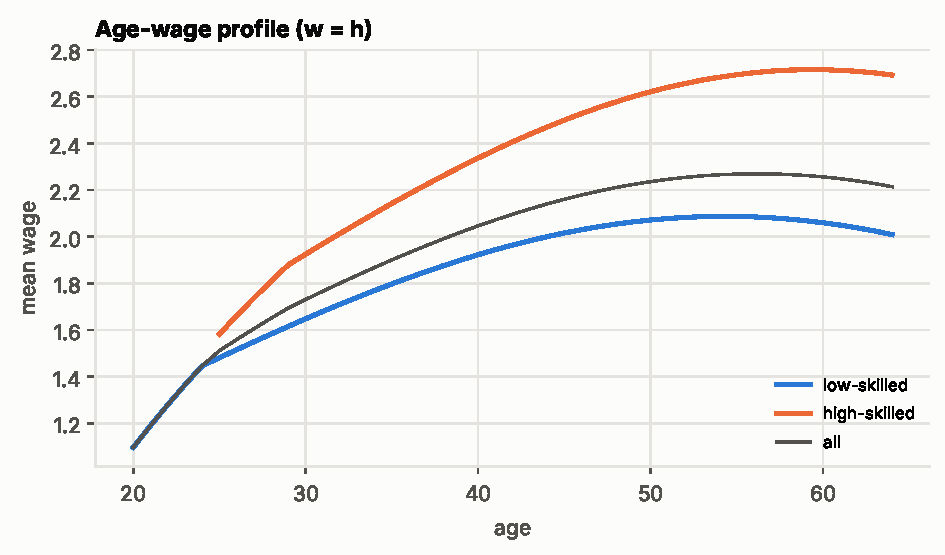
\includegraphics[width=.62\linewidth]{fig3_age_wage_profile.pdf}
\caption{Age--wage profile in the baseline. Mean over 30 replications and 60 years; bands are 95\% confidence intervals.}\label{fig:profile}
\end{figure}

\subsection{The skill cliff: a mechanism experiment}

To isolate the channel through which AI will operate, we halve $p$ permanently from year 10 onwards, holding everything else constant.\footnote{This is not an AI scenario: it is the comparative dynamics of the meeting channel alone.} Figure~\ref{fig:cohorts} reports mean human capital by age class. The response is immediate for workers aged 20--29, whose human capital is 5.6 per cent lower after four years. For senior workers the response is delayed: their mean human capital is \emph{exactly} unchanged for ten years, falls by 0.04 per cent in the eleventh, by 3.5 per cent after 25 years and by 6.7 per cent in the new steady state, while output falls by 7.1 per cent. Successive age classes start to decline roughly 15, 20--25 and 30 years after the shock.

The path of learning efficiency is non-monotonic (Figure~\ref{fig:B}, panel b). $B^{\mathrm{inc}}$ halves at impact, from 0.045 to 0.022; it then rises to 0.025 over the following two decades, because juniors start from lower levels and the gap to their seniors widens; and it falls again, to 0.021 after 50 years, as seniors trained under fewer meetings become the teachers. Learning efficiency thus inherits the history of meetings: it is not a parameter but a state variable. Finally, the wage Gini rises from 0.135 to about 0.154 (Figure~\ref{fig:gini}): meetings compress inequality by pulling juniors towards seniors.

\begin{figure}[t]\centering
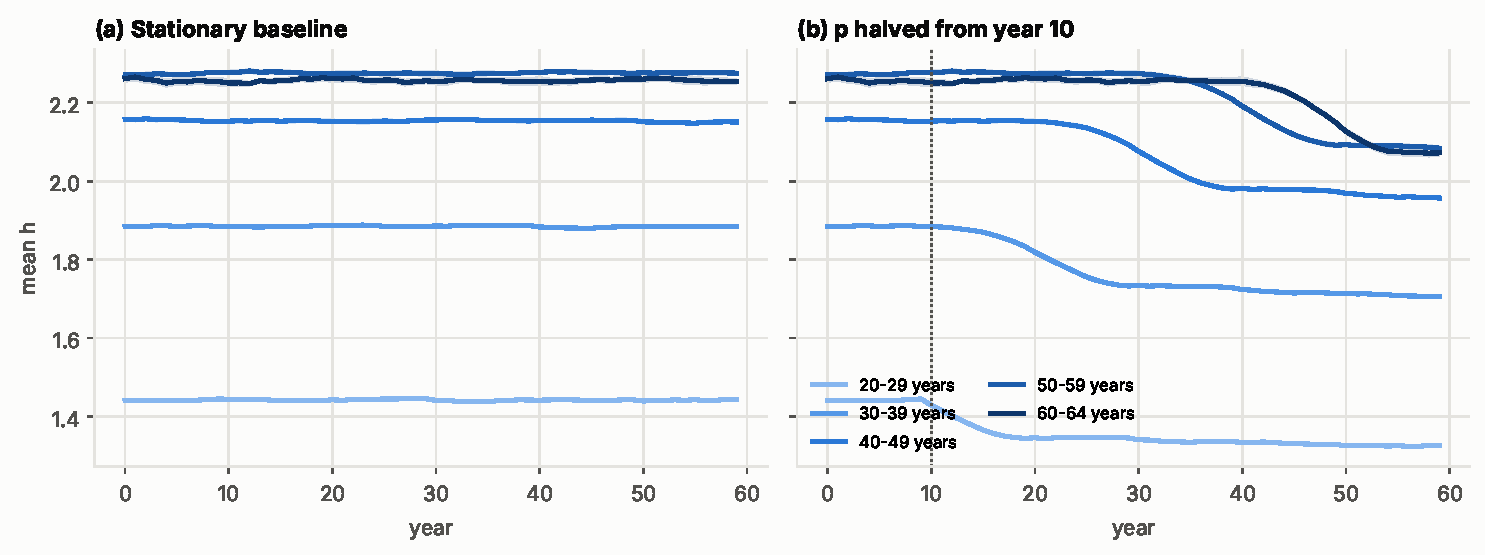
\includegraphics[width=\linewidth]{fig1_h_by_age_class.pdf}
\caption{Mean human capital by age class. (a) Baseline. (b) Meeting probability halved from year 10. Mean over 30 replications; bands are 95\% confidence intervals.}\label{fig:cohorts}
\end{figure}

\begin{figure}[t]\centering
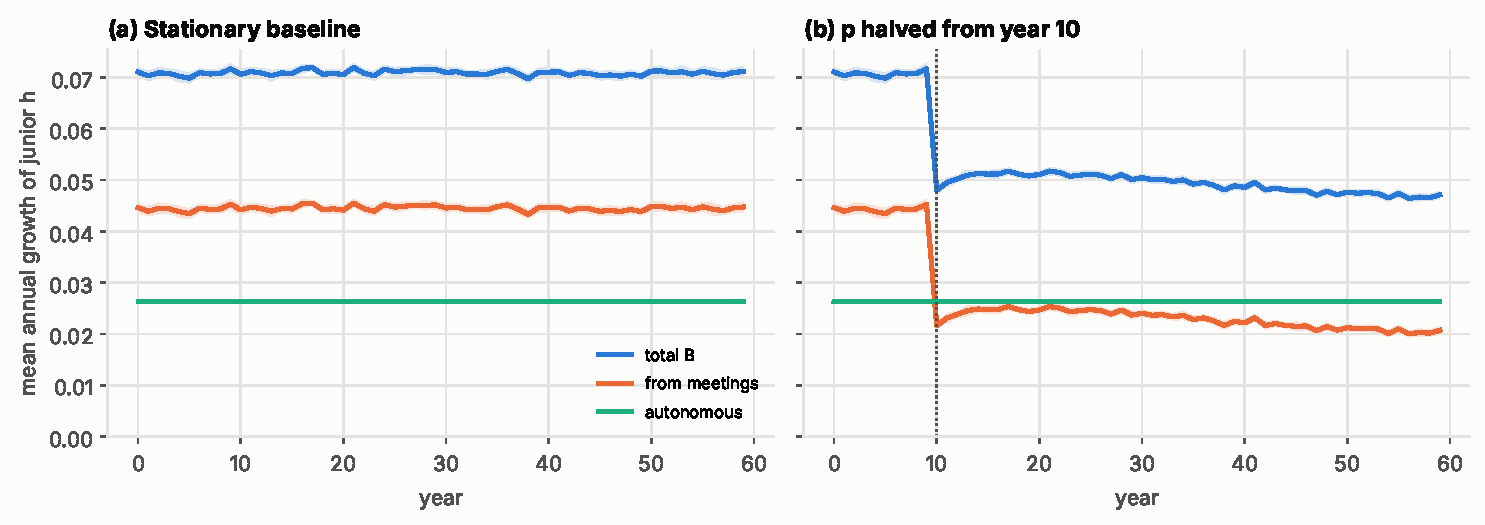
\includegraphics[width=\linewidth]{fig2_emergent_B.pdf}
\caption{Emergent learning efficiency of junior workers and its decomposition.}\label{fig:B}
\end{figure}

\begin{figure}[t]\centering
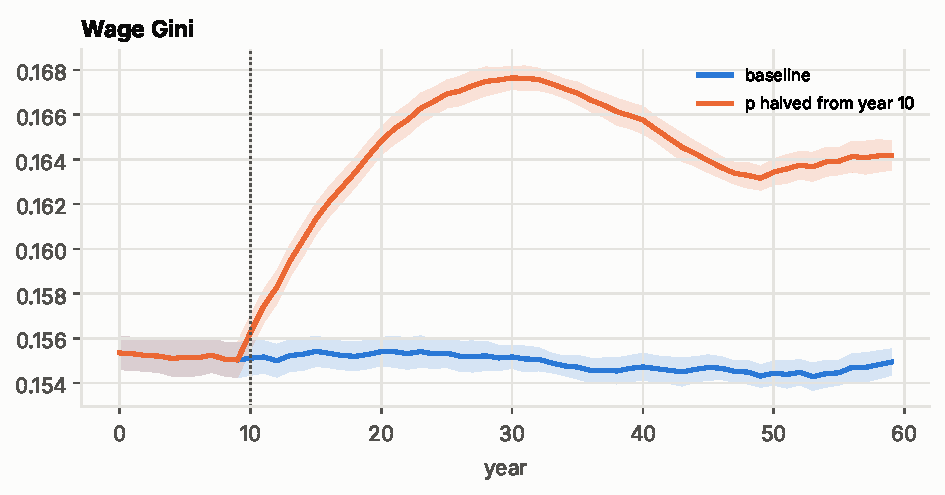
\includegraphics[width=.62\linewidth]{fig4_gini.pdf}
\caption{Wage Gini coefficient.}\label{fig:gini}
\end{figure}

\subsection{Mentoring capacity}

Figure~\ref{fig:sens} shows $B^{\mathrm{inc}}$ and mean senior human capital as functions of $p$ for different values of $\kappa$. Both increase more than linearly in $p$, reflecting the cumulative mechanism described above, until the capacity constraint in Eq.~\eqref{eq:peff} binds, at $p=\kappa S/J$; beyond that point additional demand for meetings is rationed. In the baseline the constraint becomes active only if $S/J$ falls below $p/\kappa=3$, that is, after a large reduction in the number of seniors relative to juniors.

\begin{figure}[t]\centering
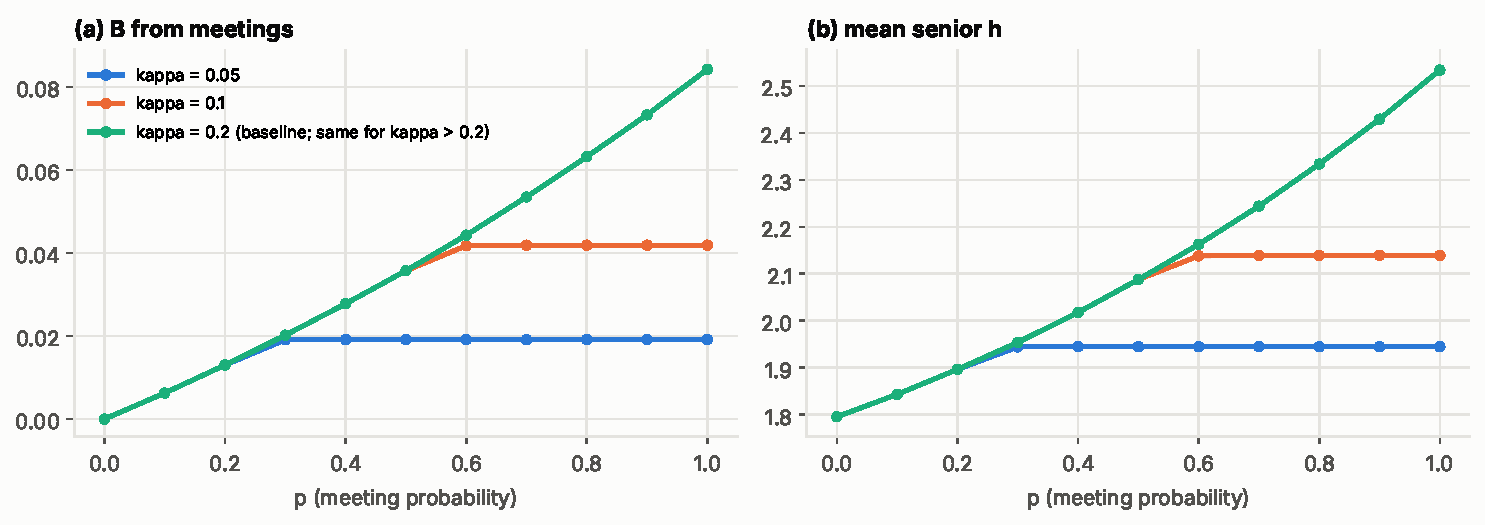
\includegraphics[width=\linewidth]{fig5_sensitivity_p_kappa.pdf}
\caption{Sensitivity to the meeting probability $p$ and to mentoring capacity $\kappa$ (10 replications per point).}\label{fig:sens}
\end{figure}

% ---------------------------------------------------------------------------
\section{Implications for aggregate modelling}\label{sec:aggregate}

Single-equation growth models remain popular, and with good reason. Are there lessons from the agent-based model that can be incorporated into them? We argue that there are two.

\begin{proposition}[Emergent learning efficiency]\label{prop:B}
Let $\bar h^S_t$ be mean senior human capital, $\overline{h^{-1}}^{J}_t$ the mean of the inverse of junior human capital, and $\bar\delta^J$ the mean autonomous learning rate of juniors, all at the beginning of period $t$. Under random matching, the expected learning efficiency of juniors is
\begin{equation}\label{eq:Bmf}
\mathbb E[B_t] = \bar\delta^J - d + \beta\, p^{\mathrm{eff}}_t \left[\bar h^S_t\, \overline{h^{-1}}^{J}_t - 1 + \Omega_t\right],
\end{equation}
where
\begin{equation*}
\Omega_t = \frac{1}{J_t S_t}\sum_{j,k}\frac{\max(0,h_{j,t}-h_{k,t})}{h_{j,t}} \ge 0 .
\end{equation*}
\end{proposition}
\begin{proof}
Since $\max(0,x) = x + \max(0,-x)$, the expected gain of junior $j$ from a meeting with a uniformly drawn senior is $\beta(\bar h^S_t - h_{j,t}) + \beta S_t^{-1}\sum_k \max(0, h_{j,t}-h_{k,t})$. Dividing by $h_{j,t}$, multiplying by $p^{\mathrm{eff}}_t$ and averaging over juniors gives the meeting term; the autonomous term follows from Eq.~\eqref{eq:aut}.
\end{proof}

Eq.~\eqref{eq:Bmf} is the aggregate counterpart of the micro-level rules. Learning efficiency depends on three objects that a fixed $B$ suppresses: meeting opportunities ($p$), mentoring capacity relative to demand ($\kappa S/J$), and the distribution of knowledge between generations ($\bar h^S \overline{h^{-1}}^J$). In the baseline the identity is verified numerically (0.0443 against a simulated 0.0441). The truncation term $\Omega_t$ is small (0.0004), while the dispersion of junior human capital matters: replacing $\overline{h^{-1}}^J$ with $1/\bar h^J$ underestimates $B^{\mathrm{inc}}$ by about 16 per cent.

\begin{proposition}[Transmission lag]\label{prop:lag}
Suppose that meeting opportunities change permanently at $t_0$ and that seniors do not learn from meetings. Then mean senior human capital is unaffected for $t \le t_0 + s_S - s_J$, and is affected from $t_0 + s_S - s_J + 1$ onwards.
\end{proposition}
\begin{proof}
A worker who is junior at $t_0$ has experience at most $s_J-1$ and becomes senior when their experience reaches $s_S$, that is, after at least $s_S-s_J+1$ years. Until then the set of seniors consists of workers whose junior years ended before $t_0$, and whose human capital evolves according to Eq.~\eqref{eq:aut} alone.
\end{proof}

With $s_J=5$ and $s_S=15$ the lag is 11 years, exactly as observed in the simulations. Proposition~\ref{prop:lag} explains why the first-round evidence on young workers \citep{Brynjolfsson2025} cannot, by itself, reveal the second-round effect on human capital: the latter is invisible for a full professional generation, and then unfolds over several. The long-run elasticity of senior human capital to meeting opportunities, $\varepsilon = \Delta \ln \bar h^S_\infty / \Delta\ln p \approx 0.10$ in the baseline, plays here the role that the degree of hysteresis plays in aggregate models of the normal rate of utilisation \citep{Bassi2022}: it summarises in a single number a property that emerges from heterogeneous micro-behaviour.

% ---------------------------------------------------------------------------
\section{Conclusions}\label{sec:conclusions}

This paper contributes to the literature in three respects. First, it shows that learning efficiency can be modelled as an emergent property of encounters between workers, and that a parsimonious agent-based model reproduces a concave age--wage profile and a plausible share of learning from coworkers. Second, it shows that a reduction in meeting opportunities produces a delayed and cumulative fall in human capital---a skill cliff---whose timing is governed by the distance between the junior and senior thresholds. Third, it provides an aggregate identity that can be used to make learning efficiency endogenous in single-equation growth models.

These contributions aside, the analysis leaves open several avenues for research. The next step is to introduce AI explicitly: a productivity index $A_t$ growing at rate $g$, a target that determines which workers are substituted (junior, senior, high-skilled, low-skilled, or none in the complementary case), a mapping from $A_t$ to the meeting probability and effectiveness, and an output function $Y_t = f(\sum_i h_{i,t}, A_t)$. The skill cliff hypothesis then becomes a race between the growth of AI productivity and the erosion of the knowledge it relies upon. A demographic variant based on the Italian age pyramid, where large cohorts approach retirement, will make it possible to separate the cliff generated by demography from the one added by AI.

The policy implications follow from Proposition~\ref{prop:lag}. If the costs of substituting junior work materialise only after a decade, they will not be reflected in the incentives of firms that adopt AI today. Mentoring and apprenticeship then acquire the character of a public good, whose under-provision is invisible in the data until it is too late to correct it cheaply.

\section*{CRediT authorship contribution statement}
\textbf{Federico Bassi:} \todo{da definire}. \textbf{\todo{Nome Cognome}:} Conceptualization, Methodology, Software, Writing -- original draft.

\section*{Data availability}
Code, configuration files and simulated data are available at \url{https://github.com/ViciusLio/skill-cliff-abm}.

\appendix
\section{Docking with an independent implementation}\label{app:docking}

Table~\ref{tab:docking} compares the vectorised model with an independent implementation in Mesa (one object per agent) with $N=1{,}000$ and 20 replications each. No difference is statistically significant.

\begin{table}[h]\centering\small
\caption{Docking: vectorised (NumPy) vs.\ object-based (Mesa) implementation.}\label{tab:docking}
\begin{tabular}{lrrrr}
\toprule
Statistic & NumPy & Mesa & Rel.\ diff. & $p$-value (Welch) \\
\midrule
Mean $h$ & 1.9900 & 1.9858 & $-0.21\%$ & 0.34 \\
Mean junior $h$ & 1.4157 & 1.4110 & $-0.33\%$ & 0.19 \\
Mean senior $h$ & 2.1652 & 2.1613 & $-0.18\%$ & 0.42 \\
$B^{\mathrm{inc}}$ & 0.0444 & 0.0444 & $+0.12\%$ & 0.86 \\
$B^{\mathrm{aut}}$ & 0.0264 & 0.0264 & $0.00\%$ & 0.76 \\
\bottomrule
\end{tabular}
\end{table}

\bibliographystyle{elsarticle-harv}
\bibliography{references}

\end{document}
